\documentclass[11pt, titlepage]{article}
\usepackage[IL2]{fontenc}
\usepackage{times}
\usepackage{bigfoot}
\usepackage{multirow}
\usepackage{pdflscape}
\usepackage{amsmath}
\usepackage{graphicx}
\usepackage{enumitem} % for line spacing in itemize
\usepackage{url}
\usepackage[a4paper, total={17cm, 24cm}, top=3cm, left=2cm]{geometry}

\graphicspath{{../}}

\begin{document}
\urlstyle{rm}
% User defined title page
\begin{titlepage}
    \begin{center}
        \textsc{\Huge{Brno University of Technology\\[0.3em]}}
        \textsc{\huge{Faculty of Information Technology}}
        
        \vspace{\stretch{0.382}}
        
        \Huge{Formal Languages and Compilers\\}
        \huge{Project documentation\\}
        \LARGE{Team 062., variant I\\}
        \Large{UNARY, BOOLTHEN}
        
        \vspace{\stretch{0.618}}
    \end{center}
    {
    		\Large{\today}{\hfill \textbf{Dominik Horky} \texttt{xhorky32} 25\% \\
    			\phantom{ }\hfill Lukas Hais \texttt{xhaisl00} 25\%\\ 
	    		\phantom{ }\hfill Roman Janiczek \texttt{xjanic25} 25\% \\
    			\phantom{ }\hfill Jan Pospisil \texttt{xpospi94} 25\% \\}
    	}
\end{titlepage}

\tableofcontents
\newpage


%%%%%%%%%%%% LEXICAL ANALYSIS %%%%%%%%%%%%%%%
\section{Lexical analysis (scanner)}\label{lexical-analysis-scanner}

\subsection{About}\label{about}

The first step of creating compiler for IFJ20 was implementing the
scanner. The scanner is implemented as a \emph{ravenous finite state
automaton} (see Figure \ref{fig:automaton}), which performs tokenization of input file. In
\texttt{scanner.c} this is implemented as one big repetitive
\texttt{while} loop which reads 1 character after another from
\texttt{stdin} and jumps between predefined \emph{states}, in switch
case, in \texttt{scanner.h} by rules specified in automaton. If scanner
reads an invalid character it stops it's action and returns \texttt{1},
which indicates error in lexical analysis, otherwise returns valid
token, which is then processed in parser, and waits for another function call from
parser to get another token from input.

\subsection{Token}\label{token}

Token is predefined structure in \texttt{scanner.h} containing 2 core
parts: \emph{TokenType} \& \emph{TokenAttribute}

\subsubsection{Token types}\label{token-types}

\begin{itemize}[itemsep=-5pt]
\item
  EOF
\item
  EOL
\item
  Empty - when scanner encounters comment
\item
  Identifier
\item
  Keyword
\item
  Integer
\item
  String
\item
  Float
\item
  Boolean - with BOOLEAN extension
\item
  Arithmetic operators (+, -, *, /)
\item
  Relational operators (==, !=, \textgreater, \textless, \textgreater=,
  \textless=)
\item
  Logical operators (\&\&, \textbar\textbar, !)
\item
  Assignment operators (=, :=, +=, \ldots) - some of which are supported
  only thanks to UNARY extension
\item
  Brackets ((, ), \{, \})
\item
  Delimiters (comma, semicolon)
\end{itemize}

\subsubsection{Token attribute}\label{token-attribute}

\begin{itemize}[itemsep=-5pt]
\item
  String
\item
  Integer
\item
  Float
\item
  Boolean - BOOLEAN extension
\item
  Keyword - there are many predefined keywords in \texttt{scanner.h},
  most of them are reserved keywords defined by IFJ20 specifications and
  \texttt{EMPTY} keyword when none of the above attributes should be
  used.
\end{itemize}

\subsection{Usage}\label{usage}

The main function of scanner will be \texttt{getToken()}, which behavior
is described in \ref{about}. The parser calls \texttt{getToken()} function which takes
token as it's parameter. If the reading was
successful, token is filled with valid
information about what it represents and then returns from function.
Function \texttt{getToken()} distinguishes between 4 return codes it can
return: 
\begin{itemize}[itemsep=-5pt]
\item
	\texttt{0} - if reading was successful and token is returned
\item
	\texttt{1} - if lexical error (determined by automaton)
\item
	\texttt{2} - if given token equals to NULL
\item
	\texttt{99} - if internal problem (ex. malloc failure)
\end{itemize}

If returned code does not equals to \texttt{0}, program should stop it's
action, clean after itself and inform user about what happened.
%%%%%%%%%%%%  END LEXICAL ANALYSIS %%%%%%%%%%%%%%%






%%%%%%%%%%%% SYNTAX ANALYSIS %%%%%%%%%%%%%%%
\section{Syntax analysis (parser)}\label{syntax-analysis-parser}

\subsection{About}\label{about-1}

Second most important part of our compiler is parser. Parser takes
token stream from scanner and,
depending on rules specified in LL table (see Figure \ref{fig:LLtable}), transforms
them into Abstract Syntax Tree (AST), which in our case is Binary
Search Tree (BST). In \texttt{parser.c} this is implemented as various
functions which acts as LL rules (see. Figure \ref{fig:LLgramar}). If token stream
taken from parser has invalid syntax, parser stops it's action and
returns \texttt{2}, which indicates error in syntax analysis, also
it can perform some necessities from semantic analysis and call \texttt{semantic\_analysis()} from \texttt{semantic.c} file and 
\texttt{precedent\_analys()} function from \texttt{precedent.h}.
\subsubsection{Syntax analysis - Top-Down parsing}\label{syntax-analysis---top-down-parsing}

For a syntax analysis we decided to use Top-Down parsing, which seemed
optimal for our case, with recursive descent parsing. The top-down
parsing performs construction of BST from root and then proceeds towards
it's leaves.

\subsubsection{Recursive Descent Parsing}\label{recursive-descent-parsing}

This parsing technique consists of few function, one for each
non-terminal in the grammar, and recursively parses the input to make a
BST tree.

\subsubsection{Parsing using precedent syntax
analysis}\label{parsing-using-precedent-syntax-analysis}

Because some expressions contain arithmetic and logical operators, we
have to check priority for those operators and evaluate correct order in
which we perform those operations. Priority for those operators are
specified by precedent table (see Figure \ref{fig:PreTable}). Precedent syntax
analysis is not part of \texttt{parser} files but is implemented in
standalone \texttt{precedent} files. At start it takes token from parser
and then, one by one, gets next tokens and determines how to correctly evaluate them.
After that they are generated to \texttt{stdin}.

\subsection{Functions}\label{functions}
In this section we only specify calling other parser's functions, not generator neither semantic analysis functions.
\begin{itemize}[itemsep=-5pt]
\item
  Parser - Main function of compiler, prepares symtable and stack for
  further usage, then calls \texttt{program}
\item
  Program - Strips comments and EOLs and then calls \texttt{prolog()},
  \texttt{eolM()} and \texttt{functionsBlock()}
\item
  Prolog - Checks whether file starts with \texttt{package\ main}
\item
  EolM - Checks whether prologue is ended with EOL and then calls
  \texttt{eolR}
\item
  EolR - Strips EOLs
\item
  FunctionsBlock - Checks that token is KEYWORD \texttt{func} and calls
  \texttt{function()} and \texttt{functionNext()}, after that checks that
  \texttt{main} function was found only once
\item
  Function - Checks that next tokens are KEYWORD \texttt{func} and IDENTIFIER, if so then it saves
  it's name to functions symtable. Then it looks for \texttt{(} and
  calls \texttt{arguments()}. If \texttt{arguments()} was successful
  and current token is \texttt{)} it calls \texttt{functionReturn()} and
  \texttt{commandBlock()}
\item
  FunctionNext - Checks if there are any other functions, if so, calls
  \texttt{function()} and \texttt{functionNext()}
\item
  Arguments - Checks whether token is IDENTIFIER, if so calls
  \texttt{type()} and \texttt{argumentNext()}
\item
  ArgumentNext - If token is comma, then perform action as
  \texttt{arguments()} function
\item
  Type - Checks whether token equals to KEYWORD \texttt{int}, \texttt{float64},
  \texttt{string} or \texttt{bool}
\item
  FunctionReturn - If token is \texttt{(} calls
  \texttt{functionReturnType()}, otherwise continue because
  return \texttt{()} could be omitted.
\item
  FunctionReturnType - If token equals to KEYWORD, calls \texttt{type()}
  and \texttt{functionReturnTypeNext()} and then looks for \texttt{)}, if
  it equals to \texttt{)}, continue with program
\item
  FunctionReturnTypeNext - Checks that token is COMMA, another token
  should be KEYWORD and calls \texttt{type()} and
  \texttt{functionReturnTypeNext()}
\item
  CommandBlock - Checks that token is \texttt{\{}, then gets another
  which should be EOL, if so strips remaining EOLs. If next token does
  not equal to \texttt{\}}, calls \texttt{commands()} and then checks that
  token equals to \texttt{\}}, then look for one required EOL, if it's not after 
  if statement, and strip remaining EOLs
\item
  Commands - Calls \texttt{command()}, checks that command is ended with
  EOL, strips remaining EOLs and then determines whether token equals to
  \texttt{\}}, if so returns result, otherwise calls \texttt{commands()}
\item
  Command - Contains switch statement which determines next action. If
  token equals to IDENTIFIER calls \texttt{statement()}. If token equals
  to KEYWORD go to another switch statement determining what kind of
  action we should perform based on passed KEYWORD:

  \begin{itemize}[itemsep=-5pt]
  \item
    IF - calls \texttt{commandBlock()} and \texttt{ifElse()} functions
  \item
    FOR - calls \texttt{forDefine()} and then checks that token equals to
    \texttt{;}, after that calls \texttt{commandBlock()}
  \item
    RETURN - calls \texttt{returnCommand()}
  \item
    default - invalid KEYWORD passed
  \end{itemize}
\item
  Statement - Contains another switch statement which distinguishes
  between those token types:

  \begin{itemize}[itemsep=-5pt]
  \item
    \texttt{(} - calls \texttt{funcCallArguments()} function and checks that token
    equals to \texttt{EOL}
  \item
    \texttt{=} - calls \texttt{assignment()} function
  \item
    \texttt{:=} - calls generator's and precedent's functions
  \item
    \texttt{+=}, \texttt{-=}, \texttt{*=}, \texttt{/=} - calls
    \texttt{unary()} function
  \item
    default - calls \texttt{multipleID()}, then checks that token equals
    to \texttt{=} and calls \texttt{assignment()}
  \end{itemize}
\item
  MultipleID - Checks that token equals to COMMA, increases number of
  IDs, then checks that next token is IDENTIFIER and calls
  \texttt{multipleID()}
\item
  Assignment - calls \texttt{expressionNext()} after some necessary checks
\item
  Unary - Only checks that token is unary type
\item
  ExpressionNext - Checks whether token equals to COMMA, then checks
  that number of IDs - 1 is greater than 0, then calls
  \texttt{expresssionNext()} function
\item
  FuncCallArguments - performs some checks on arguments and then calls \texttt{expressionNext()}
\item
  IfElse - If token is KEYWORD and equals to ELSE then it calls
  \texttt{ifElseExpanded()} function
\item
  IfElseExpanded - If token equals to IF KEYWORD then calls
  \texttt{commandBlock()} and \texttt{ifElse()} functions, otherwise calls
  \texttt{commandBlock()} only
\item
  ForDefine - Checks that token's type equals to IDENTIFIER, if so
  checks whether next token equals to \texttt{:=}
\item
  ForAssign - Determines whether token is IDENTIFIER and next token is
  \texttt{=}
\item
  ReturnCommand - Checks that token is KEYWORD RETURN and calls
  \texttt{returnStatement}
\item
  ReturnStatement - loops through return values and assigns them
\end{itemize}

\subsection{Usage}\label{usage-1}

The only function which program should call is \texttt{program()}, which
calls other functions as it progresses through
token stream (see \ref{functions-1}). If no syntax error is
found while parsing tokens, go through stack of
symtables and calls semantic analyzer's function \texttt{semantic\_analysis} (see \ref{semantic-analysis}). Parser is
able to return various codes:

\begin{itemize}[itemsep=-5pt]
\item
  \texttt{0} - if everything was successful
\item
  \texttt{1} - if lexical error
\item
  \texttt{2} - if syntax error
\item
  \texttt{3} - if semantic error in program (undefined function,
  variable, \ldots)
\item
  \texttt{4} - if semantic error in type assignment to new variable
\item
  \texttt{5} - if semantic error in type compatibility (arithmetics,
  \ldots)
\item
  \texttt{6} - if semantic error in program (invalid number of params or
  return values)
\item
  \texttt{7} - if other semantic error
\item
  \texttt{9} - if zero division
\item
  \texttt{99} - if internal error
\item
  \texttt{-1} - if internal warning
\end{itemize}
%%%%%%%%%%%% END SYNTAX ANALYSIS %%%%%%%%%%%%%%%



%%%%%%%%%%%% SEMANTIC ANALYSIS %%%%%%%%%%%%%%%
\section{Semantic analysis}\label{semantic-analysis}

\subsection{About}\label{about-2}

Semantic analysis is run after parser checks correct
syntax of sequence of tokens and checks the semantic of it. For example
valid data types, valid return types and existence of passed
identifiers. Semantic analysis is performed right away in parser, but when we evaluate function call we use \texttt{semantic\_analysis} function defined in \texttt{semantic.c} file.
\subsection{Function}\label{function_sym}
\begin{itemize}
\item Semantic\_analysis - Check if is function is present in Global Stack, if so check if number of return values equals number of variables and then cycle through them and check their types, otherwise set number of IDs to 0
\end{itemize}
%%%%%%%%%%%% END SEMANTIC ANALYSIS %%%%%%%%%%%%%%%




%%%%%%%%%%%% CODEGEN ANALYSIS %%%%%%%%%%%%%%%
\section{Code Generator}\label{code-generator}

\subsection{About}\label{about-3}

Code generator's functions are called from parser when
specific criterion is met and it generates \emph{IFJcode20} code
depending on what we are currently generating and it sends it to
\texttt{stdout}. If everything were generated correctly we are able to
send it to interpreter (which was written by our dear professors) and
run it.

\subsection{Functions}\label{functions-1}

\begin{itemize}[itemsep=-5pt]
\item
  GenerateHeader - generates header required by ic20int and jump to main
  function
\item
  GenerateFunction - generates beginning of function or entire function
  code if it's internal function (if internal, label starts with
  \texttt{\_}, otherwise \texttt{\$})
\item
  GenerateFuncArguments - generates function's arguments and pops them
  from stack
\item
  GenerateFuncCall - generates call for specified function
\item
  GenerateFuncReturn - generates pushes of return values to stack
\item
  GenerateFuncEnd - generates end of function (return to last
  instruction and frame pop)
\item
  GenerateDefinitions - generates definition of variable
\item
  GenerateAssignments - generates variable's assignment
\item
  GeneratorPrint - generates internal function for printing, outputs 1
  argument to \texttt{stdout}
\item
  GenerateIfScope - generates \texttt{if}, \texttt{else\ if},
  \texttt{else} scope
\item
  GenerateIfScopeEnd - generates end for \texttt{if} statement}
\item
  GenerateForBeginning - generates counter variable definition
\item
  GenerateForExpression - generates assignment + expression of
  \texttt{for} loop
\item
  GenerateForCondition - generates condition for ending \texttt{for}
  loop
\item
  GenerateForAssignment - generates label of \texttt{for} assignment
\item
  GenerateForAssignmentEnd - generates jump to \texttt{for} expression
  (after assignment is done)
\item
  GenerateForScope - generates beginning of \texttt{for} loop scope
\item
  GenerateForScopeDefinitions - generates definitions of \texttt{for} loop
\item
  GenerateForScopeEnd - generates end of \texttt{for} loop scope
\item
  IgnoreIfScope - determines whether \texttt{if}, \texttt{else\ if} or
  \texttt{else} scope will be ignored and not generated
\item
  GeneratorSaveID - adds identifier to end of list for definition or
  assignment
\item
  GeneratorGetID - gets last added identifier
\item
  GenerateUsedInternalFunctions - generates used internal functions (if
  none, don't generate)
\item
  GeneratorPrintCheck - check that printArguments is true, if so pop +
  print the value to stdout, otherwise do nothing
\item
  GeneratorUnaryPrepare - pushes ID to local frame
\item
  GenerateUnaryExpression - generates instructions base on given unary type
\item
  GenerateCodeInternal - generates internal code (internal function
  code, header)
\item
  SetUpCodeInternal - sets up code variable for generating internal
  function code
\item
  IsFuncInternal - checks that given name is really internal function
\end{itemize}

\subsection{Usage}\label{usage-2}

In contrast with scanner or parser we
don't call just one function here, which would then proceed to call
other functions, but we have to call corresponding function to where we
are currently in parser and what we need to generate. For that function
names should be great indicator to know what to use.
%%%%%%%%%%%% END CODEGEN %%%%%%%%%%%%%%%





%%%%%%%%%%%% ALGO %%%%%%%%%%%%%%%
\section{Algorithms and data
structures}\label{algorithms-and-data-structures}

Due to specifications in assignment we had to create some special
data structures.

\subsection{Binary Search Tree (BST)}\label{binary-search-tree-bst}

We have implemented an Abstract Syntax Tree, which type is BST. Thanks
to second homework from IAL, all of us had to implement this, so we
scraped everything from those homeworks and created new file which suits
our needs in this case. More about this could be found in
\texttt{symtable} header and c file.

\subsection{Symbol stack}\label{symbol-stack}

We also need a stack for symbols to use in our compiler. It has few
functions that performs \emph{initialization, pushing, poping and
freeing} the stack. For more detailed info see \texttt{symstack}
files

\subsection{Dynamic string}\label{dynamic-string}

Because scanner needs to save characters to string, we are unable to use
just plain C \texttt{char} data type, so we downloaded \texttt{str}
header and c file from \texttt{jednoduchy\_intrpreter} archive which was
passed down upon us from our dear professors. This allowed us using it as
dynamic string. We also tweaked this file a bit, so it suits our exact needs.
%%%%%%%%%%%% END ALGO %%%%%%%%%%%%%%%




%%%%%%%%%%%% TEAMWORK %%%%%%%%%%%%%%%
\section{Teamwork}\label{teamwork}

\subsection{Versioning system}\label{versioning-system}

We decided that the best option for hosting our code and so will be
using github repository, so we created one, set rules about merging to
master and started developing in our own branches on parts of compiler
that were assigned to us. Every time someone wanted to push some changes
to master, he created \emph{pull request} and other teammates had to do
review on this code before merging.

\subsection{Communication}\label{communication}

For communication between teammates and few meetings, we decided for
using Discord, where we created our own server. The decision was pretty
simple, because all of us already have been using discord and were
comfortable with it.

\subsection{Who did what}\label{who-did-what}

\begin{itemize}[itemsep=-5pt]
\item
  \emph{Dominik Horky} - Team Leader, parser, generator, symtable, LL
  grammar, makefile
\item
  \emph{Roman Janiczek} - Parser, symtable, code review, github guru
\item
  \emph{Lukas Hais} - Scanner, scanner's automaton, code review,
  documentation, presentation
\item
  \emph{Jan Pospisil} - Precedent, expression, generator
\end{itemize}
%%%%%%%%%%%% END TEAMWORK %%%%%%%%%%%%%%%





%%%%%%%%%%%% OVERVIEW %%%%%%%%%%%%%%%
\section{Overview}\label{overview}

\subsection{Compiling}\label{compiling}

We have decided to write our own makefile, which we used for compiling
our source code, because none of us had experience with using
\emph{CMake} and also it was specified in assignment to be able to
compiler our program with \texttt{make} command in terminal. We also
added some other parts as \texttt{make\ debug} used when debugging code,
\texttt{make\ tests} which make tests for \emph{symtable} and
\texttt{make\ clean} that deletes everything that other \\\texttt{make\ *}
commands created.

\subsection{About project}\label{about-project}

This project seemed at first as too big bite to swallow, but as we
progressed through it with blindly writing code, finding research
materials online and watching IFJ/IAL lectures, we were able to slowly
make some parts work. The main problem in our group was probably that we
missed a lot of deadlines that we prepared for ourselves throughout time
we had until final deadline, so in the end we found ourselves with
little to no time and a few broken things either not working correctly
or not working at all, but probably performed well in the end.
%%%%%%%%%%%% END OVERVIEW %%%%%%%%%%%%%%%


\begin{center}
	\begin{figure}
		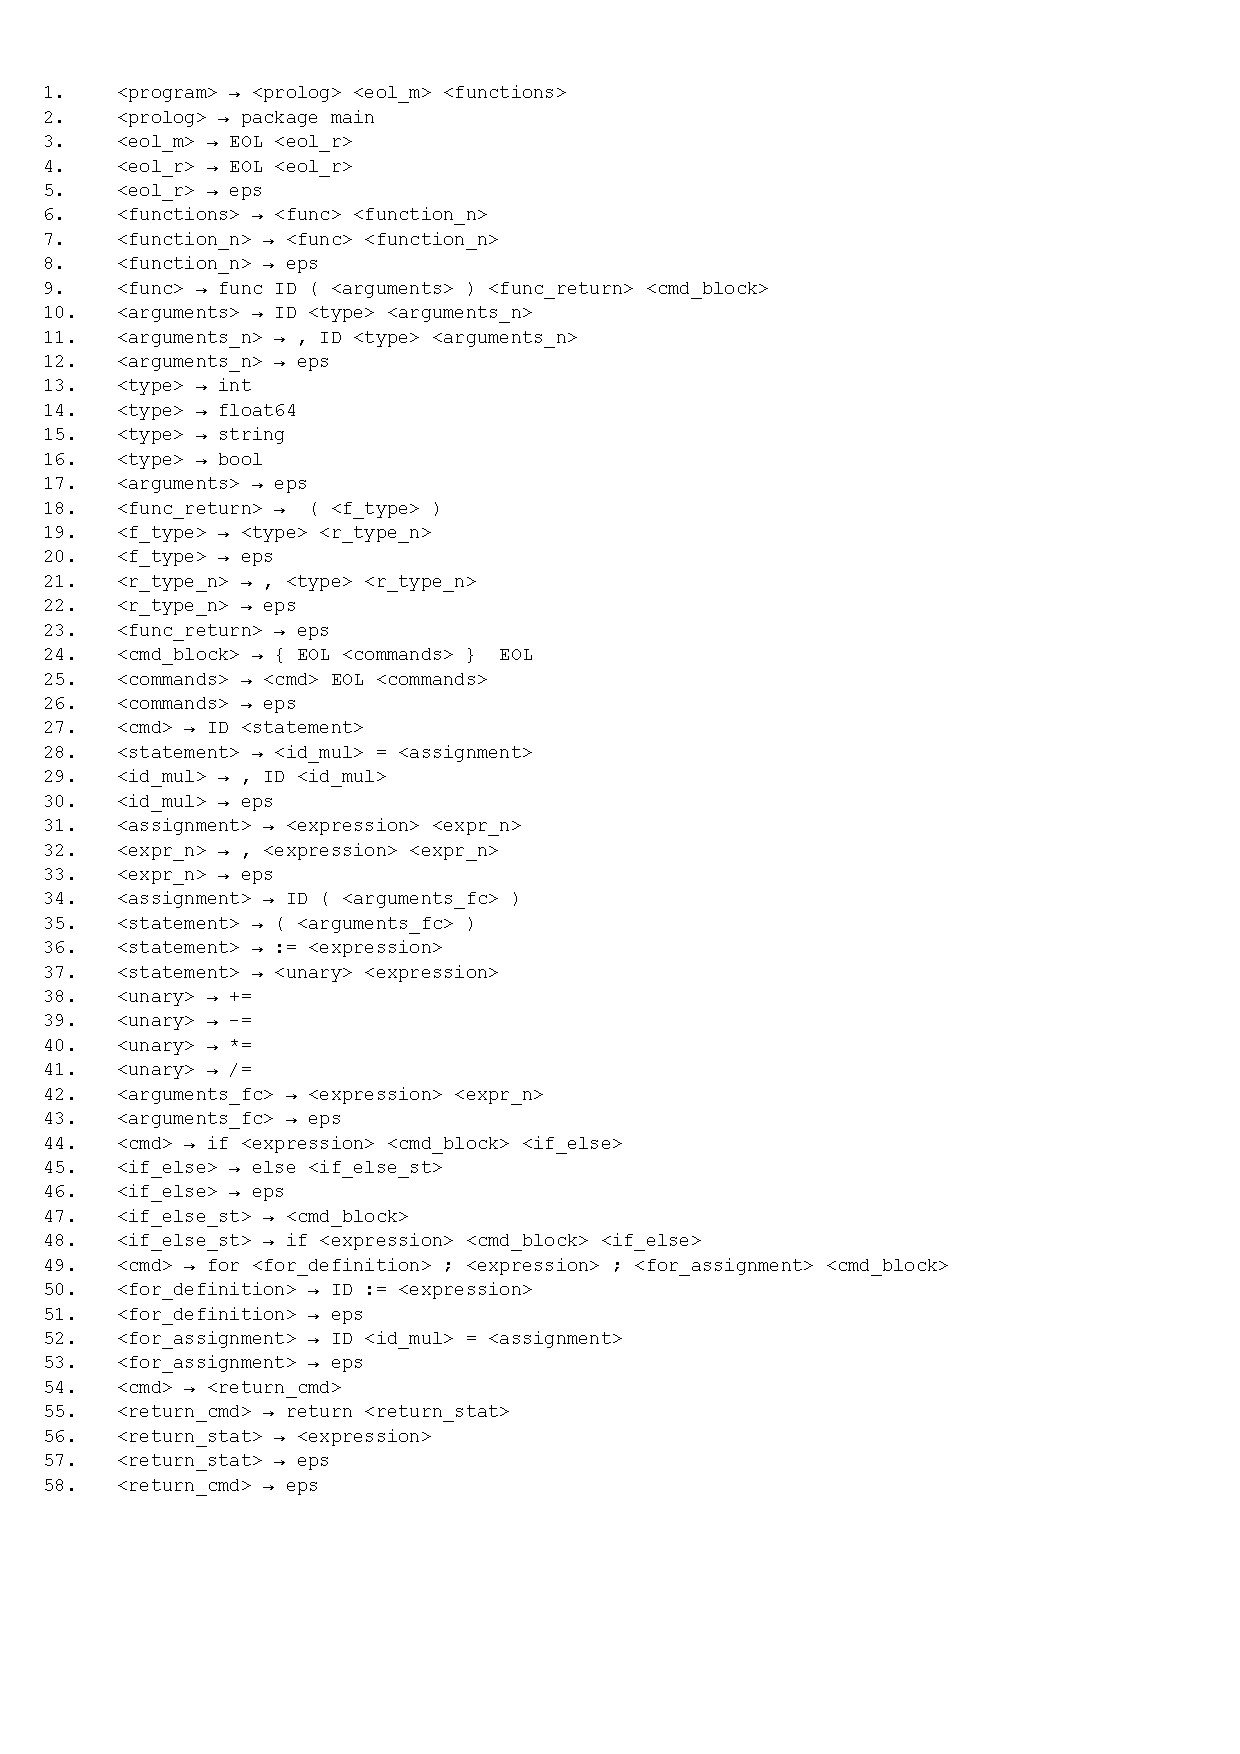
\includegraphics[width=\linewidth, height=650pt]{LL_grammar}
		\caption{LL grammar}
		\label{fig:LLgramar}
	\end{figure}
\end{center}

\begin{center}
	\begin{figure}
		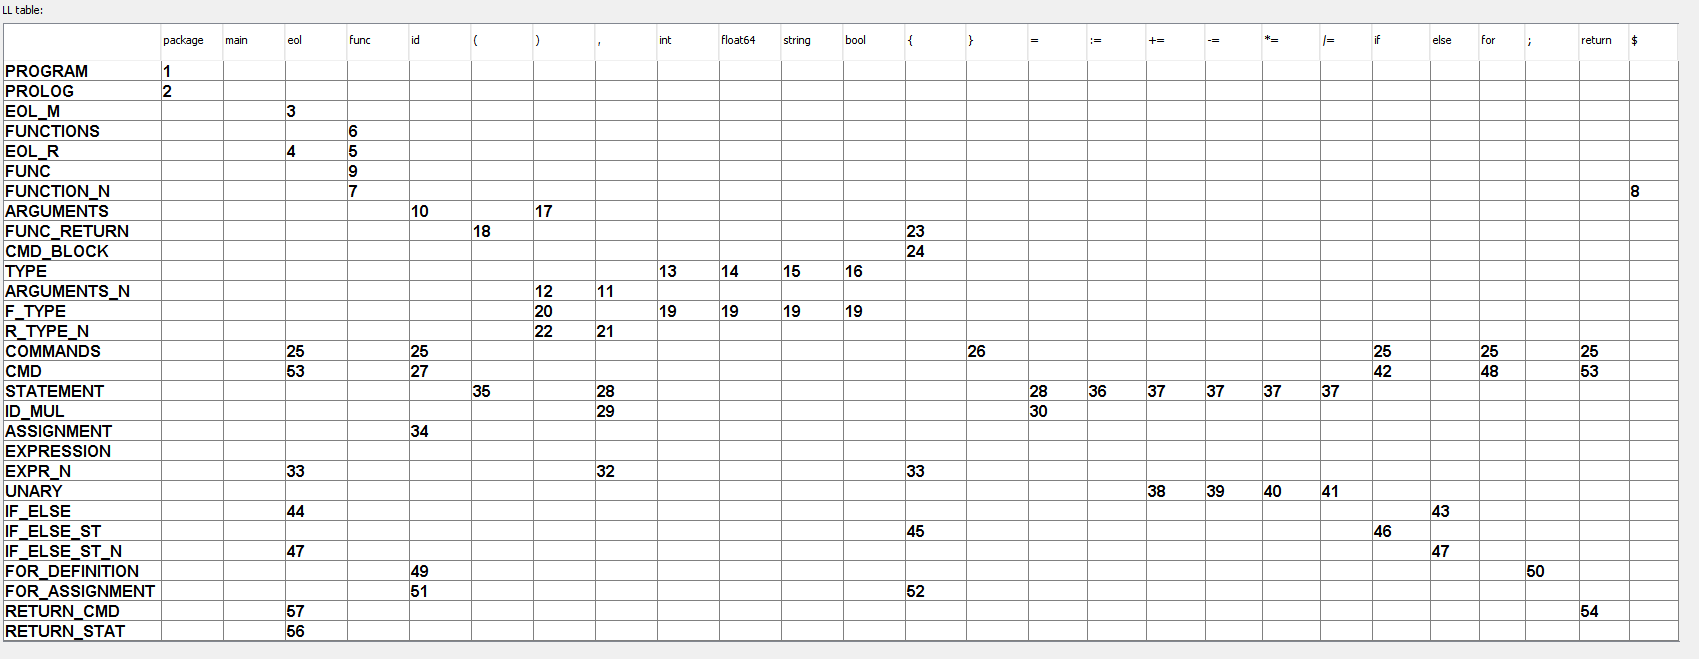
\includegraphics[width=\linewidth]{LL_table}
		\caption{LL grammar table}
		\label{fig:LLtable}
	\end{figure}
\end{center}

\begin{center}
	\begin{figure}
		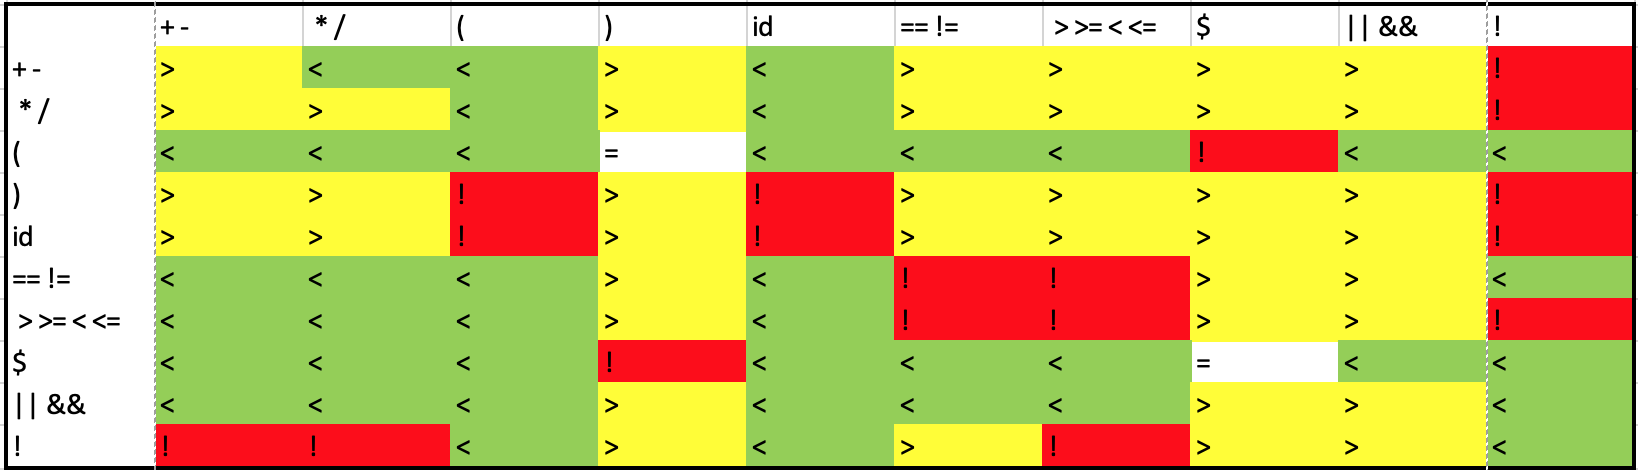
\includegraphics[width=\linewidth]{precedent}
		\caption{Precedent table}
		\label{fig:PreTable}
	\end{figure}
\end{center}

\begin{center}
	\begin{landscape}
	\begin{figure}
		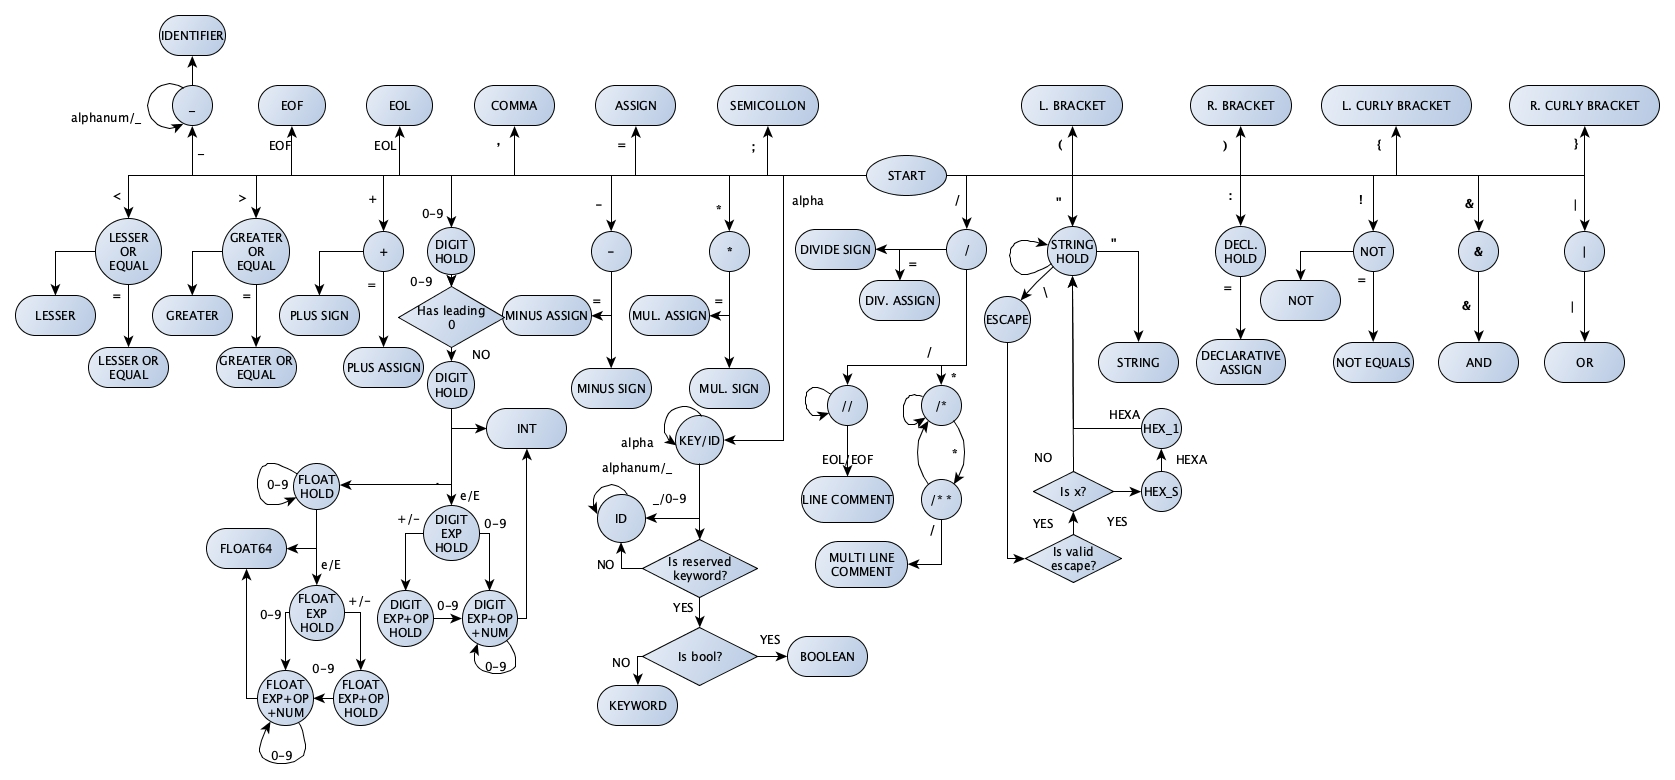
\includegraphics[width=\linewidth]{scannerAutomaton}
		\caption{Scanner\'s automaton}
		\label{fig:automaton}
	\end{figure}
	\end{landscape}
\end{center}
\end{document}
